\chapter[A Proposta de Trabalho]{A Proposta de Trabalho}

\section[Definição da Proposta]{Definição da Proposta}

Neste trabalho foi apresentado um arcabouço teórico relacionado à contratação de serviços de TI em organizações públicas brasileiras. Também foram apresentados os principais conceitos Lean na Manufatura, Lean no Desenvolvimento de \textit{Software}, Metodologias Ágeis.

À luz do levantamento bibliográfico realizado, não foram encontrados estudos que buscassem levantar e analisar os aspectos advindos do uso de metodologias ágeis em contraposição ao uso de metodologias tradicionais no contexto da gestão de contratos de fornecedores de desenvolvimento de \textit{software} para organizações públicas brasileiras.

Assim, a proposta deste trabalho consiste na investigação, coleta, análise e discussão dos resultados, de dados de contratações de fornecedores de desenvolvimento de \textit{software} por uma instituição pública brasileira. A partir da análise  dos dados será realizada uma comparação entre os resultados obtidos com uso de metodologias ágeis e os resultados obtidos sem o uso de metodologias ágeis na gestão de contratos de fornecedores de desenvolvimento de \textit{software}. O foco será a investigação da utilização das ferramentas Kanban e Scrum na fase de Gerenciamento do Contrato.


\section[Estudo de Caso]{Estudo de Caso}

O órgão público selecionado foi o Instituto do Patrimônio Histórico e Artístico Nacional (IPHAN).

O escopo do estudo de caso está ilustrado na Fig. (17). 
\begin{figure}[H]
		\centering
		\label{fig01}
			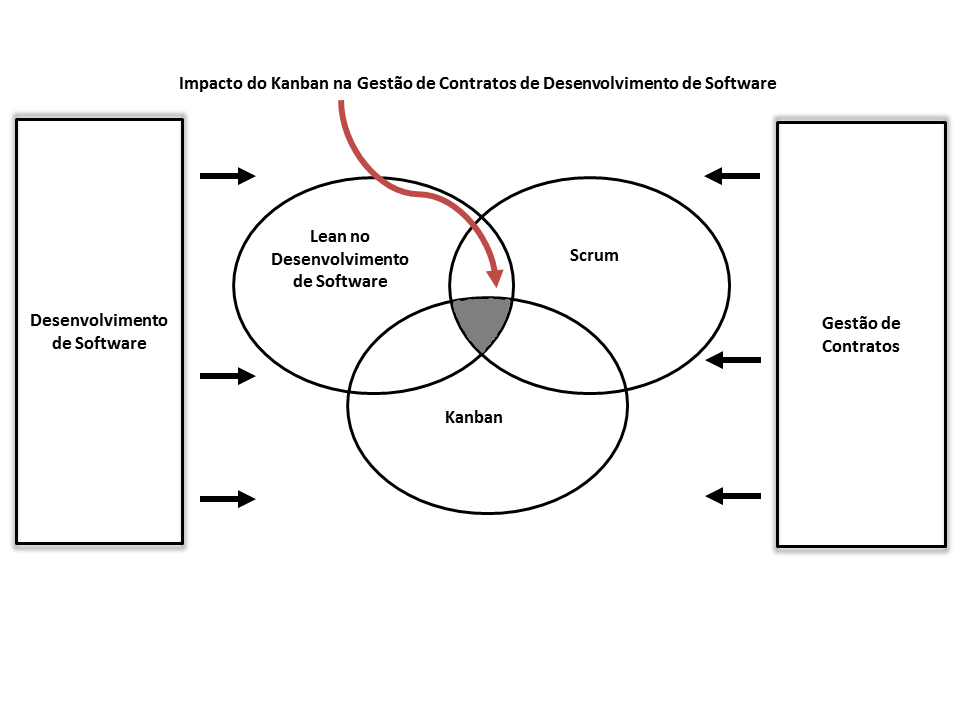
\includegraphics[scale=0.6]{figuras/escopoEC.png}
		\caption{Escopo do Estudo de Caso}
\end{figure}

\subsection[A Organização]{A Organização}

O órgão escolhido, IPHAN, possui uma força de trabalho atuante na área de TI de apenas 8 funcionários, dos quais apenas 3 trabalham diretamente com sistemas. O perfil dessa equipe é apresentado na Tab. (3). Devido ao número reduzido de servidores disponíveis na área de TI do órgão, frequentemente uma mesma pessoa acaba desempenhando diferentes papeis requeridos pela Instrução Normativa MP/SLTI Nº04/2010.

\begin{table}[H]
\center
\footnotesize
\begin{tabular}{|c|c|c|}
\hline
\textbf{Área}          & \textbf{Perfil}   & \textbf{Quantidade} \\ \hline
TI Geral               & Coordenador de Tecnologia da Informação   & 1                   \\ \hline
Infraestrutura         & Analista de Tecnologia da Informação   & 2                   \\ \hline
Sistemas               & Analista de Tecnologia da Informação   & 2                   \\ \hline
\multirow{3}{*}{Apoio} & Analista de Tecnologia da Informação    & 1                   \\ \cline{2-3} 
\multicolumn{1}{|l|}{} & Servidor do Ministério da Ciência, Tecnologia e Inovação & 1                   \\ \cline{2-3} 
\multicolumn{1}{|l|}{} & Servidor do IPHAN & 1                   \\ \hline
\end{tabular}
\caption{Perfil da Equipe}
\end{table}

O contexto atual do órgão foi identificado por meio da aplicação da técnica de entrevista semi-estruturada. A estrutura da entrevista pode ser encontrada no Apêndice I -  Roteiro de Entrevista.

Os fatores mais significantes que são gerenciados pela área de TI do órgão, segundo o entrevistado, são:
\begin{itemize}
\item Atender as demandas para desenvolvimento de sistemas (sistema novo, manutenção, documentação).
\item Controlar de qualidade de sistemas.
\item Possuir medições de sistemas.
\end{itemize}

Por meio da entrevista foram identificados alguns problemas, dentre eles:
\begin{itemize}
\item Alguns contratos foram encerrados sem haver entrega de \textit{software};
\item Havia faturamento de Ordens de Serviço apenas com entrega de documentação;
\item Incapacidade de aferir a qualidade interna do produto;
\item As mudanças de requisitos geravam impacto no tempo de execução do projeto, ocasionando constantes atrasos.
\end{itemize}

A partir dos problemas identificados, ainda conforme o entrevistado, as principais motivações para o uso de metodologias ágeis na gestão de contratos foram: aumentar o volume de entregas \textit{software}; prover maior visibilidade do processo e do produto para o do gestor de negócio; empoderar o gestor do contrato sobre a gerência dos requisitos, de forma a eliminar  a interferência direta do gestor de contrato e, por fim, perceber de forma mais rápida se o projeto terá sucesso ou não, pois os riscos inerentes à contratação poderiam ser identificados com antecedência.

Conforme apresentado no capítulo 4 o IPHAN possui uma Metodologia de Gestão de Demandas de Desenvolvimento de \textit{Software} (MIDAS), detalhada no Anexo B, além de um Kanban para Gestão destas Demandas. 

De acordo com a Instrução Normativa MP/SLTI Nº04/2010, a fase de Gerenciamento de Contrato deve conter as seguintes etapas: início do contrato; encaminhamento formal de ordem de serviço ou fornecimento de bens  monitoramento da execução; e transição contratual e/ou encerramento do contrato. Todas estas etapas podem estão contempladas no MIDAS, fazendo com que ele seja aderente ao normativo e adequado para o estudo de caso deste trabalho.

De acordo com o entrevistado, as metas norteadoras para a elaboração do MIDAS foram:
\begin{itemize}
\item Ser aderente à legislação pertinente;
\item Entregar \textit{software} mais rapidamente;
\item Focar na gestão do contrato e na definição de uma metodologia de gestão de demandas;
\item Não focar em dizer como a empresa deveria desenvolver o \textit{software}, ou seja, não definir metodologia de desenvolvimento de \textit{software};
\item Satisfazer as necessidades do cliente.
\end{itemize}

Outros instrumentos contratuais que foram modificados com o uso do MIDAS foram a forma de pagamento e a aplicação de multas. Em relação a esta, diferentemente das outras formas de gestão de contrato utilizadas anteriormente, onde as multas eram progressivamente aplicadas, por exemplo, sobre a não entrega de documentação somente além de deter caráter meramente punitivo. Com o MIDAS, passou-se a considerar o maturidade e crescimento da empresa no contrato e as multas eram somente aplicadas se não houvesse entrega de \textit{software}. O faturamento das ordens de serviço era executado a cada entrega, final de \textit{sprint}, com duração mensal, o que mantinha o fluxo de caixa da empresa contratada sempre ativo.

\subsection[Hipóteses]{Hipóteses}

Para investigar e responder a questão de pesquisa definida na seção 1.3 do Capítulo 1 - Introdução, algumas hipóteses serão analisadas:
\begin{itemize}
\item  A utilização de Metodologias Ágeis combinadas com o Lean no Desenvolvimento de Software, na gestão de contratos públicos, diminui a quantidade de contratos que são finalizados com sucesso;
\item  A utilização de Metodologias Ágeis combinadas com o Lean no Desenvolvimento de Software, na gestão de contratos públicos, aumenta o tempo para entrega de software;
\item	A satisfação do cliente com o resultado da contratação é menor com a utilização de Metodologias Ágeis combinadas com o Lean no Desenvolvimento de Software na gestão de contratos;
\item  O custo final do contrato no que diz respeito às horas de trabalho dos servidores que são pagas é maior com a utilização de Metodologias Ágeis combinadas com o Lean no Desenvolvimento Software na gestão de contratos;
\item  O processo para autorização de uma mudança no software leva mais tempo com a utilização de Metodologias Ágeis combinadas com o Lean no Desenvolvimento de Software na gestão de contratos;
\item	A quantidade de multas aplicadas na gestão de contratos é maior com a utilização de Metodologias Ágeis combinadas com o Lean no Desenvolvimento de Software;
\item	A quantidade de documentação desnecessária entregue para o gestor do contrato e para o órgão é maior com a utilização de Metodologias Ágeis combinadas com o Lean no Desenvolvimento Software;
\item  A qualidade do produto gerado com a utilização de Metodologias Ágeis combinadas com o Lean no Desenvolvimento de Software na gestão de contratos é menor.
\end{itemize}

\subsection[Fonte e Método Coleta de Dados]{Fonte e Método de Coleta de Dados}

Os dados serão coletados por meio de entrevistas semiestruturadas e por meio da análise de documentos de cerca de quatro contratos que serão disponibilizados pelo órgão. Os contratos disponibilizados estarão relacionados aos seguintes sistemas:
\begin{itemize}
\item  O contrato do Sistema Integrado de Conhecimento e Gestão (SICG) com a empresa EGL - Engenharia, no qual foram utilizadas metodologias ágeis para gestão do contrato;
\item  O contrato do Fiscalis com a empresa Velp Tecnologia, no qual foi utilizado o MPS-BR como base da gestão do contrato;
\item  O contrato do SIGIPHAN com a empresa Gestão TI, no qual não foi utilizado qualquer metodologia na gestão do contrato;
\item  O contrato com a empresa Squadra que desempenhou o papel de "fábrica" de software, desenvolvendo projetos diversos, no qual foi utilizado o Rational Unified Process (RUP) para gestão do contrato.
\end{itemize}

\section[Resultados Esperados]{Resultados Esperados}

Neste trabalho espera-se ter como resultado uma análise comparativa entre o uso de Metodologias Ágeis combinadas com o Lean Software e sem o uso destas metodologias na gestão de contratos de fornecedores de desenvolvimento de software baseada nas hipóteses definidas.

A partir das hipóteses, espera-se 

\section[Cronograma de Execução]{Cronograma de Execução}

O cronograma de marcos definido para atingir o objetivo desse trabalho com as atividades já realizadas e com as atividades futuras para o trabalho final é apresentado na Fig. (18). 

\begin{figure}[H]
		\centering
		\label{fig02}
			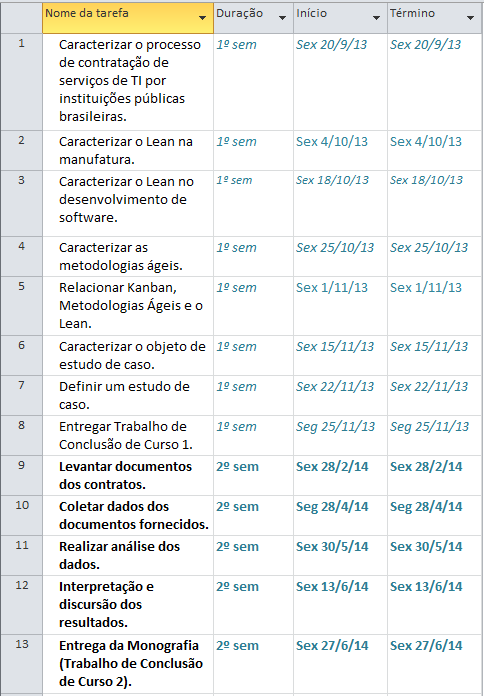
\includegraphics[scale=1.0]{figuras/cronograma3.png}
		\caption{Cronograma de Marcos}
\end{figure}

 \vspace{\onelineskip}
 \vspace{\onelineskip}
A Figura (19) apresenta uma Estrutura Analítica do Projeto com os pacotes entregáveis desse trabalho.

\begin{figure}[H]
		\centering
		\label{fig02}
			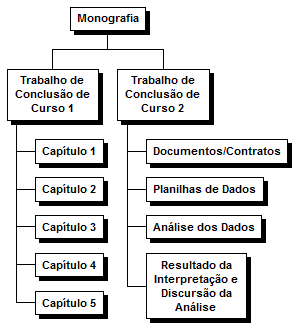
\includegraphics[scale=1.0]{figuras/wbs.png}
		\caption{Estrutura Analítica do Projeto}
\end{figure}